\begin{example}[Définition 10 : $a > b$ : $a = 7$, $b = 3$]
    ~
    \begin{itemize}
        \item Limites pour toute séquence de $\mathcal{PF}_{7,3}$
            une fois triée : $[1,\ 1 \frac{3}{7},\ 1 \frac{6}{7},\ 
            2 \frac{2}{7},\ 2 \frac{5}{7},\ 3 \frac{1}{7},\ 
            3 \frac{4}{7}]$
        \item $f_1 = (2, 1, 1, 3, 2, 3, 1) \in
            \mathcal{PF}_{7,3}$
        \item $f_2 = (2, 1, 2, 3, 2, 3, 1) \notin
            \mathcal{PF}_{7,3}$, bien que $f_2 \in
            \mathcal{PF}_7$
    \end{itemize}
\end{example}

\begin{example}[Définition 10 : $a < b$ : $a = 5$, $b = 7$]
    ~
    \begin{itemize}
        \item Limites pour toute séquence de $\mathcal{PF}_{5,7}$
            une fois triée : $[1,\ 2 \frac{2}{5},\ 3 \frac{4}{5},\ 
            5 \frac{1}{5},\ 6 \frac{3}{5}]$
        \item $f_3 = (6, 3, 5, 1, 2) \in
            \mathcal{PF}_{5,7}$, bien que $f_3 \notin
            \mathcal{PF}_5$
        \item $f_4 = (6, 3, 5, 1, 3) \notin
            \mathcal{PF}_{5,7}$\\
    \end{itemize}
\end{example}

\begin{example}[Théorème 6 : $a = 3, b = 5$]
    ~\\
    \begin{itemize*}\\
        \item $pf_{a,b} = 25$
        \item Limites : $[1,\ 2 \frac{2}{3},\ 
            4 \frac{1}{3}]$\\\\
        \subitem $(1, 1, 1)$
        \subitem $(1, 1, 2)$
        \subitem $(1, 1, 3)$
        \subitem $(1, 1, 4)$
        \subitem $(1, 2, 1)$
        \subitem $(1, 2, 2)$
        \subitem $(1, 2, 3)$
        \subitem $(1, 2, 4)$
        \subitem $(1, 3, 1)$
        \subitem $(1, 3, 2)$
        \subitem $(1, 4, 1)$
        \subitem $(1, 4, 2)$
        \subitem $(2, 1, 1)$
        \subitem $(2, 1, 2)$
        \subitem $(2, 1, 3)$
        \subitem $(2, 1, 4)$
        \subitem $(2, 2, 1)$
        \subitem $(2, 3, 1)$
        \subitem $(2, 4, 1)$
        \subitem $(3, 1, 1)$
        \subitem $(3, 1, 2)$
        \subitem $(3, 2, 1)$
        \subitem $(4, 1, 1)$
        \subitem $(4, 1, 2)$
        \subitem $(4, 2, 1)$\\
    \end{itemize*}
\end{example}

\begin{example}[Définition 11 : $a > b : a = 7, b = 3$]
    ~\\
    \begin{align*}
        &w_1 = 1110011110 \text{ n'est \emph{pas} un 7, 3 - mot de
        Dyck, car } |11100|_1 = 3\\
        & \hspace{5cm} < \frac{7}{3}|11100|_0
        = \frac{14}{3} = 4 \frac{1}{3}.\\
        &w_2 = 1110111010 \text{ \emph{est} un 7, 3 - mot de Dyck : }\\
    \end{align*}
    
\begin{center}
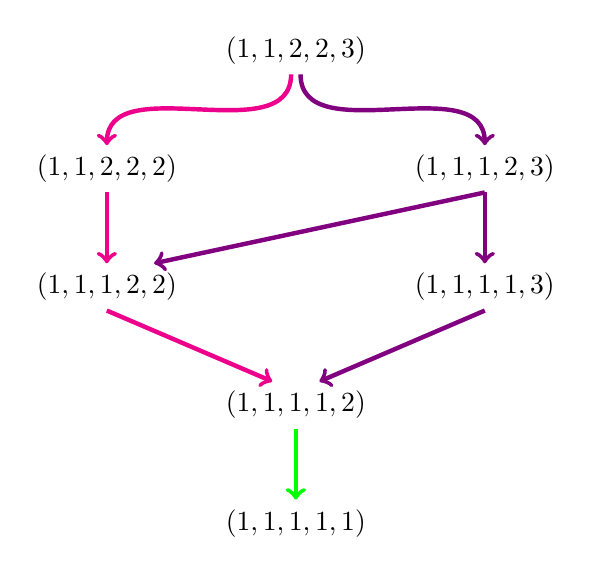
\begin{tikzpicture}[scale = 0.3]
    \node at (0,0) {$(1, 1, 1, 1, 1)$};

    \node at (0,5) {$(1, 1, 1, 1, 2)$};
        
    \node at (-8,10) {$(1, 1, 1, 2, 2)$};
    \node at (8,10)  {$(1, 1, 1, 1, 3)$};

    \node at (-8,15) {$(1, 1, 2, 2, 2)$};
    \node at (8,15)  {$(1, 1, 1, 2, 3)$};

    \node at (0,20) {$(1, 1, 2, 2, 3)$};

    \draw [->][out=-90,in=90, ultra thick] 
        [color=magenta](-0.2,19) to (-8,16);
    \draw [->][color=magenta, ultra thick]
        (-8,14) to (-8,11);
    \draw [->][color=magenta, ultra thick]
        (-8,9) to (-1,6);        

    \draw [->][out=-90,in=90, ultra thick] 
        [color=green](0,4) to (0,1);

    \draw [->][out=-90,in=90, ultra thick]
        [color=violet](0.2,19) to (8,16);
    \draw [->][color=violet, ultra thick]
        (8,14) to (-6,11);
    \draw [->][color=violet, ultra thick]
        (8,14) to (8,11);
    \draw [->][color=violet, ultra thick]
        (8,9) to (1,6);

\end{tikzpicture}
\end{center}
\end{example}

\begin{example}[Définition 11 : $a < b : a = 3, b = 5$]
    ~\\
    \begin{align*}
        &w_1 = 10100010 \text{ n'est \emph{pas} un 3, 5 - mot de
        Dyck, car } |101000|_1 = 2\\
        & \hspace{5cm} < \frac{3}{5}|101000|_0
        = \frac{12}{5} = 2 \frac{2}{5}.\\
        &w_2 = 10100100 \text{ \emph{est} un 3, 5 - mot de Dyck : }\\
    \end{align*}
    \begin{center}
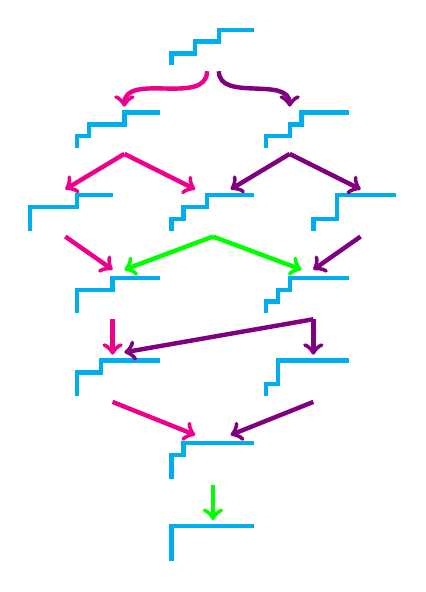
\begin{tikzpicture}[scale = 0.15]
    \draw [ultra thick, color = cyan] (0,0) -- (0,1)
        -- (0,2) -- (0,3) -- (1,3) -- (2,3) -- (3,3)
        -- (4,3) -- (5,3) -- (6,3) -- (7,3);

    \draw [ultra thick, color = cyan] (0,7) -- (0,8)
        -- (0,9) -- (1,9) -- (1,10) -- (2,10) -- (3,10)
        -- (4,10) -- (5,10) -- (6,10) -- (7,10);

    \draw [ultra thick, color = cyan] (-8,14) -- (-8,15)
        -- (-8,16) -- (-7,16) -- (-6,16) -- (-6,17) -- (-5,17)
        -- (-4,17) -- (-3,17) -- (-2,17) -- (-1,17);
        
    \draw [ultra thick, color = cyan] (8,14) -- (8,15)
        -- (9,15) -- (9,16) -- (9,17) -- (10,17)
        -- (11,17) -- (12,17) -- (13,17) -- (14,17)
        -- (15,17);

    \draw [ultra thick, color = cyan] (-8,21) -- (-8,22)
        -- (-8,23) -- (-7,23) -- (-6,23) -- (-5,23)
        -- (-5,24) -- (-4,24) -- (-3,24) -- (-2,24)
        -- (-1, 24);

    \draw [ultra thick, color = cyan] (8,21) -- (8,22)
        -- (9,22) -- (9,23) -- (10,23) -- (10,24) -- (11,24)
        -- (12,24) -- (13,24) -- (14,24) -- (15,24);

    \draw [ultra thick, color = cyan] (-12,28) -- (-12,29)
        -- (-12,30) -- (-11,30) -- (-10,30) -- (-9,30) -- (-8,30)
        -- (-8,31) -- (-7,31) -- (-6,31) -- (-5,31);

    \draw [ultra thick, color = cyan] (0,28) -- (0,29)
        -- (1,29) -- (1,30) -- (2,30) -- (3,30) -- (3,31)
        -- (4,31) -- (5,31) -- (6,31) -- (7,31);

    \draw [ultra thick, color = cyan] (12,28) -- (12,29)
        -- (13,29) -- (14,29) -- (14,30) -- (14,31) -- (15,31)
        -- (16,31) -- (17,31) -- (18,31) -- (19,31);

    \draw [ultra thick, color = cyan] (-8,35) -- (-8,36)
        -- (-7,36) -- (-7,37) -- (-6,37) -- (-5,37) -- (-4,37)
        -- (-4,38) -- (-3,38) -- (-2,38) -- (-1,38);

    \draw [ultra thick, color = cyan] (8,35) -- (8,36)
        -- (9,36) -- (10,36) -- (10,37) -- (11,37) -- (11,38)
        -- (12,38) -- (13,38) -- (14,38) -- (15,38);

    \draw [ultra thick, color = cyan] (0,42) -- (0,43)
        -- (1,43) -- (2,43) -- (2,44) -- (3,44) -- (4,44)
        -- (4,45) -- (5,45) -- (6,45) -- (7,45);

    \draw [->][out=-90,in=90, ultra thick] 
        [color=magenta](3,41.5) to (-4,38.5);
    \draw [->][color=magenta, ultra thick]
        (-4,34.5) to (-9,31.5);
    \draw [->][color=magenta, ultra thick]
        (-4,34.5) to (2,31.5);        
    \draw [->][color=magenta, ultra thick]
        (-9,27.5) to (-5,24.7);
    \draw [->][color=magenta, ultra thick]
        (-5,20.5) to (-5,17.5);
    \draw [->][color=magenta, ultra thick]
        (-5,13.5) to (2,10.7);

    \draw [->][color=green, ultra thick]
        (3.5,27.5) to (-4,24.7);
    \draw [->][color=green, ultra thick]
        (3.5,27.5) to (11,24.7);
    \draw [->][out=-90,in=90, ultra thick] 
        [color=green](3.5,6.5) to (3.5,3.5);

    \draw [->][out=-90,in=90, ultra thick]
        [color=violet](4,41.5) to (10,38.5);
    \draw [->][color=violet, ultra thick]
        (10,34.5) to (5,31.5);
    \draw [->][color=violet, ultra thick]
        (10,34.5) to (16,31.5);
    \draw [->][color=violet, ultra thick]
        (16,27.5) to (12,24.7);
    \draw [->][color=violet, ultra thick]
        (12,20.5) to (-4,17.7);
    \draw [->][color=violet, ultra thick]
        (12,20.5) to (12,17.5);
    \draw [->][color=violet, ultra thick]
        (12,13.5) to (5,10.7);

\end{tikzpicture}
\end{center}
\end{example}